\chapter{Results and Discussion}

\section[XRD analysis of diffraction spectra]{X-ray diffraction analysis of diffraction spectra of fabricated films}

X-ray diffraction patterns of thin films were analyzed using Match!, an x-ray diffraction analysis software.
It was determined using the program and the Crystallography Open Database that the films fabricated using S1 and S3 have similar diffraction patterns to zinc oxide using the database, while the thin films fabricated using S2 show little to no similarity with zinc oxide.
Figure \ref{fig:xrd} shows the diffraction pattern of the films. It can be observed that there are strong observable peaks at $2\theta$ angles $32\degg$, $34\degg$, and $36\degg$ for S1 (blue) and S3 (green), which is similar to the pattern of zinc oxide \cite{gao08}.
It can also be observed that there are little to know observable peaks in the diffraction pattern of S2 (orange).

\begin{figure}
  \centering
  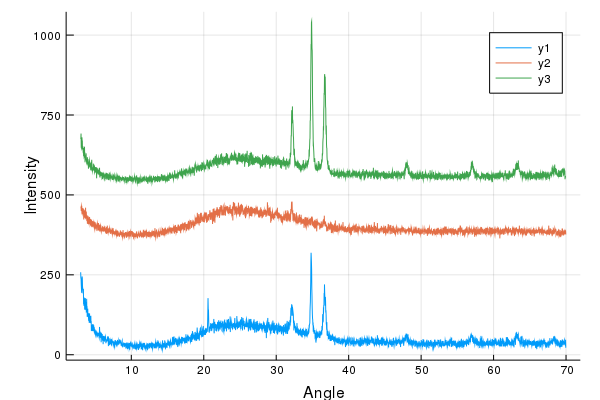
\includegraphics[scale=0.5]{xrd.png}
  \caption{X-ray diffraction spectra of fabricated thin films}
  \label{fig:xrd}
\end{figure}

Since there were little to no diffraction peaks visible and a wide curve (glass structure) in the diffraction pattern of S2 from Figure \ref{fig:xrd}, this suggests that there was little to no material or growth in the substrate.
This may be since the glass surface was not conducive for ionic adhesion in few deposition cycles as compared to S1 and S3 \cite{gao08}.
It can be seen that thermal annealing increased the crystallinity of structures as can be noted by the peak height difference between S1 and S3.
This means that the particles have arranged themselves to the desired orientation through solid state diffusion \cite{fdoping}.

\section{Qualitative differences in film structure}

Three sets of thin films have been fabricated from three varying successive ionic layer adhesion and reaction processes.
Shown in Figure \ref{fig:hpo} are some of the images that were captured using the high power objective lens of a digital compound microscope.

\begin{figure}
  \centering
  \begin{subfigure}{.4\textwidth}
    \centering
    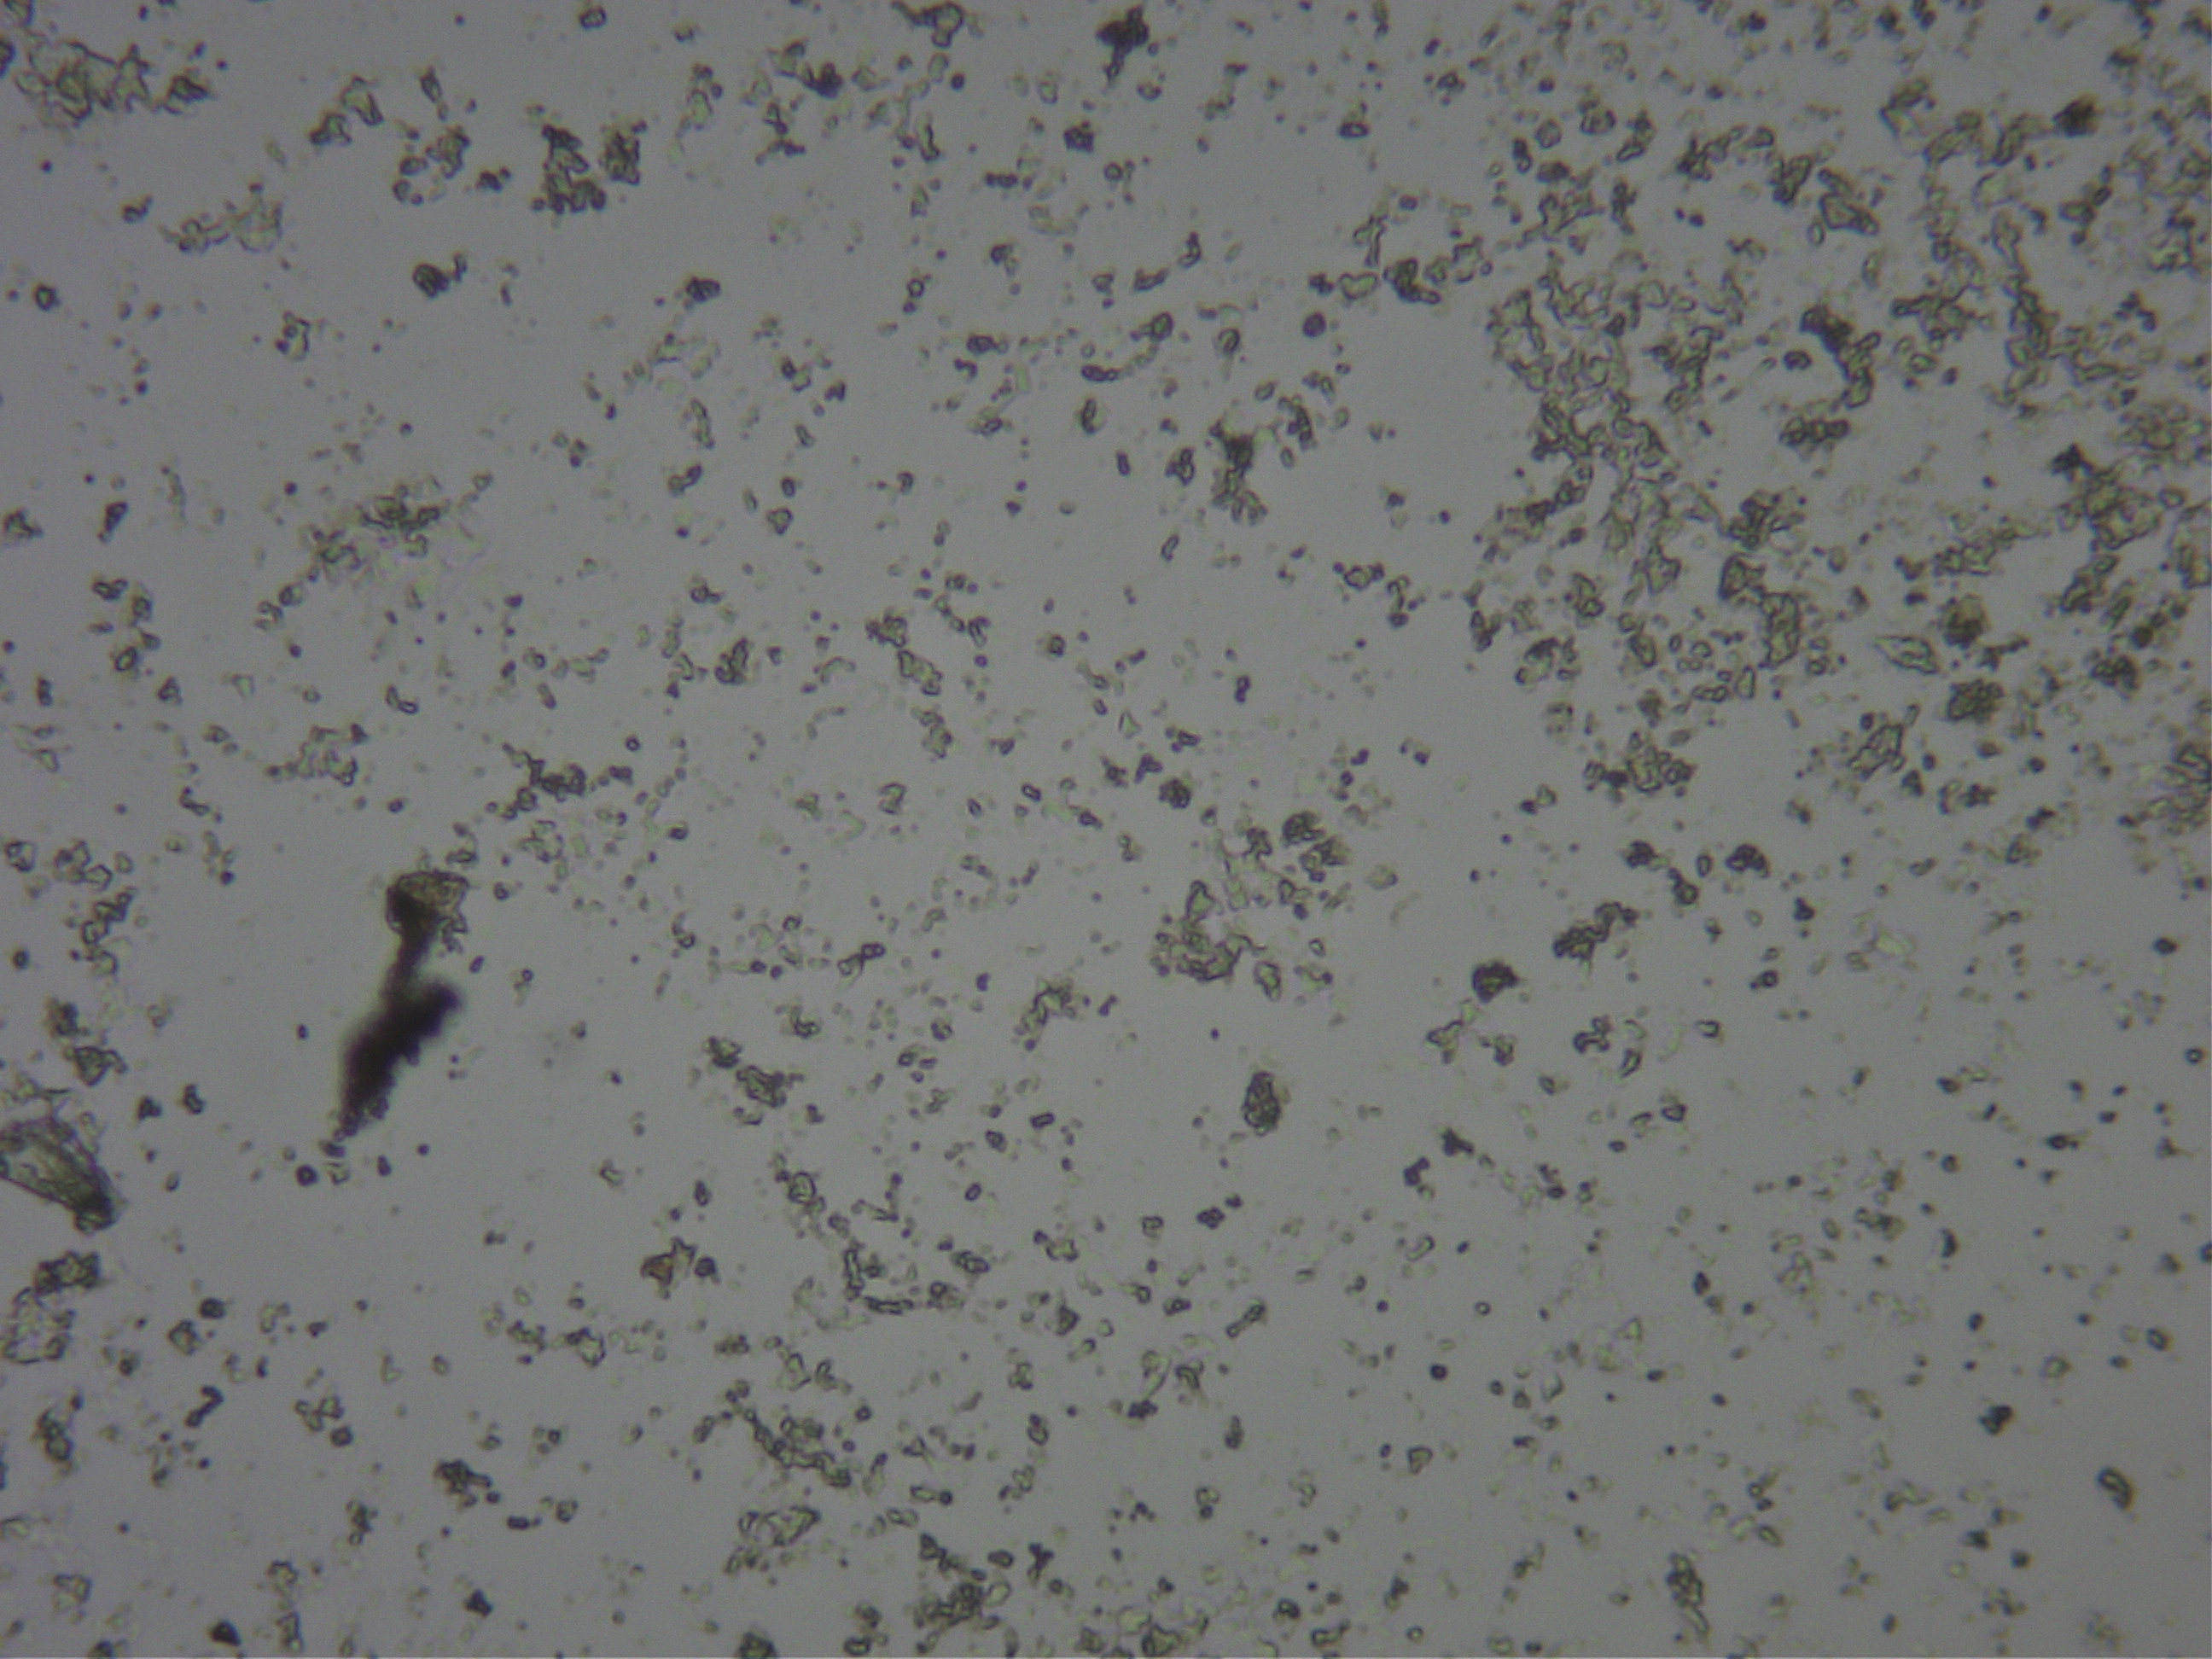
\includegraphics[scale=0.065]{s2.JPG}
    \caption{Dark clumps present in thin films}
    \label{fig:dark}
  \end{subfigure}
  \begin{subfigure}{.4\textwidth}
    \centering
    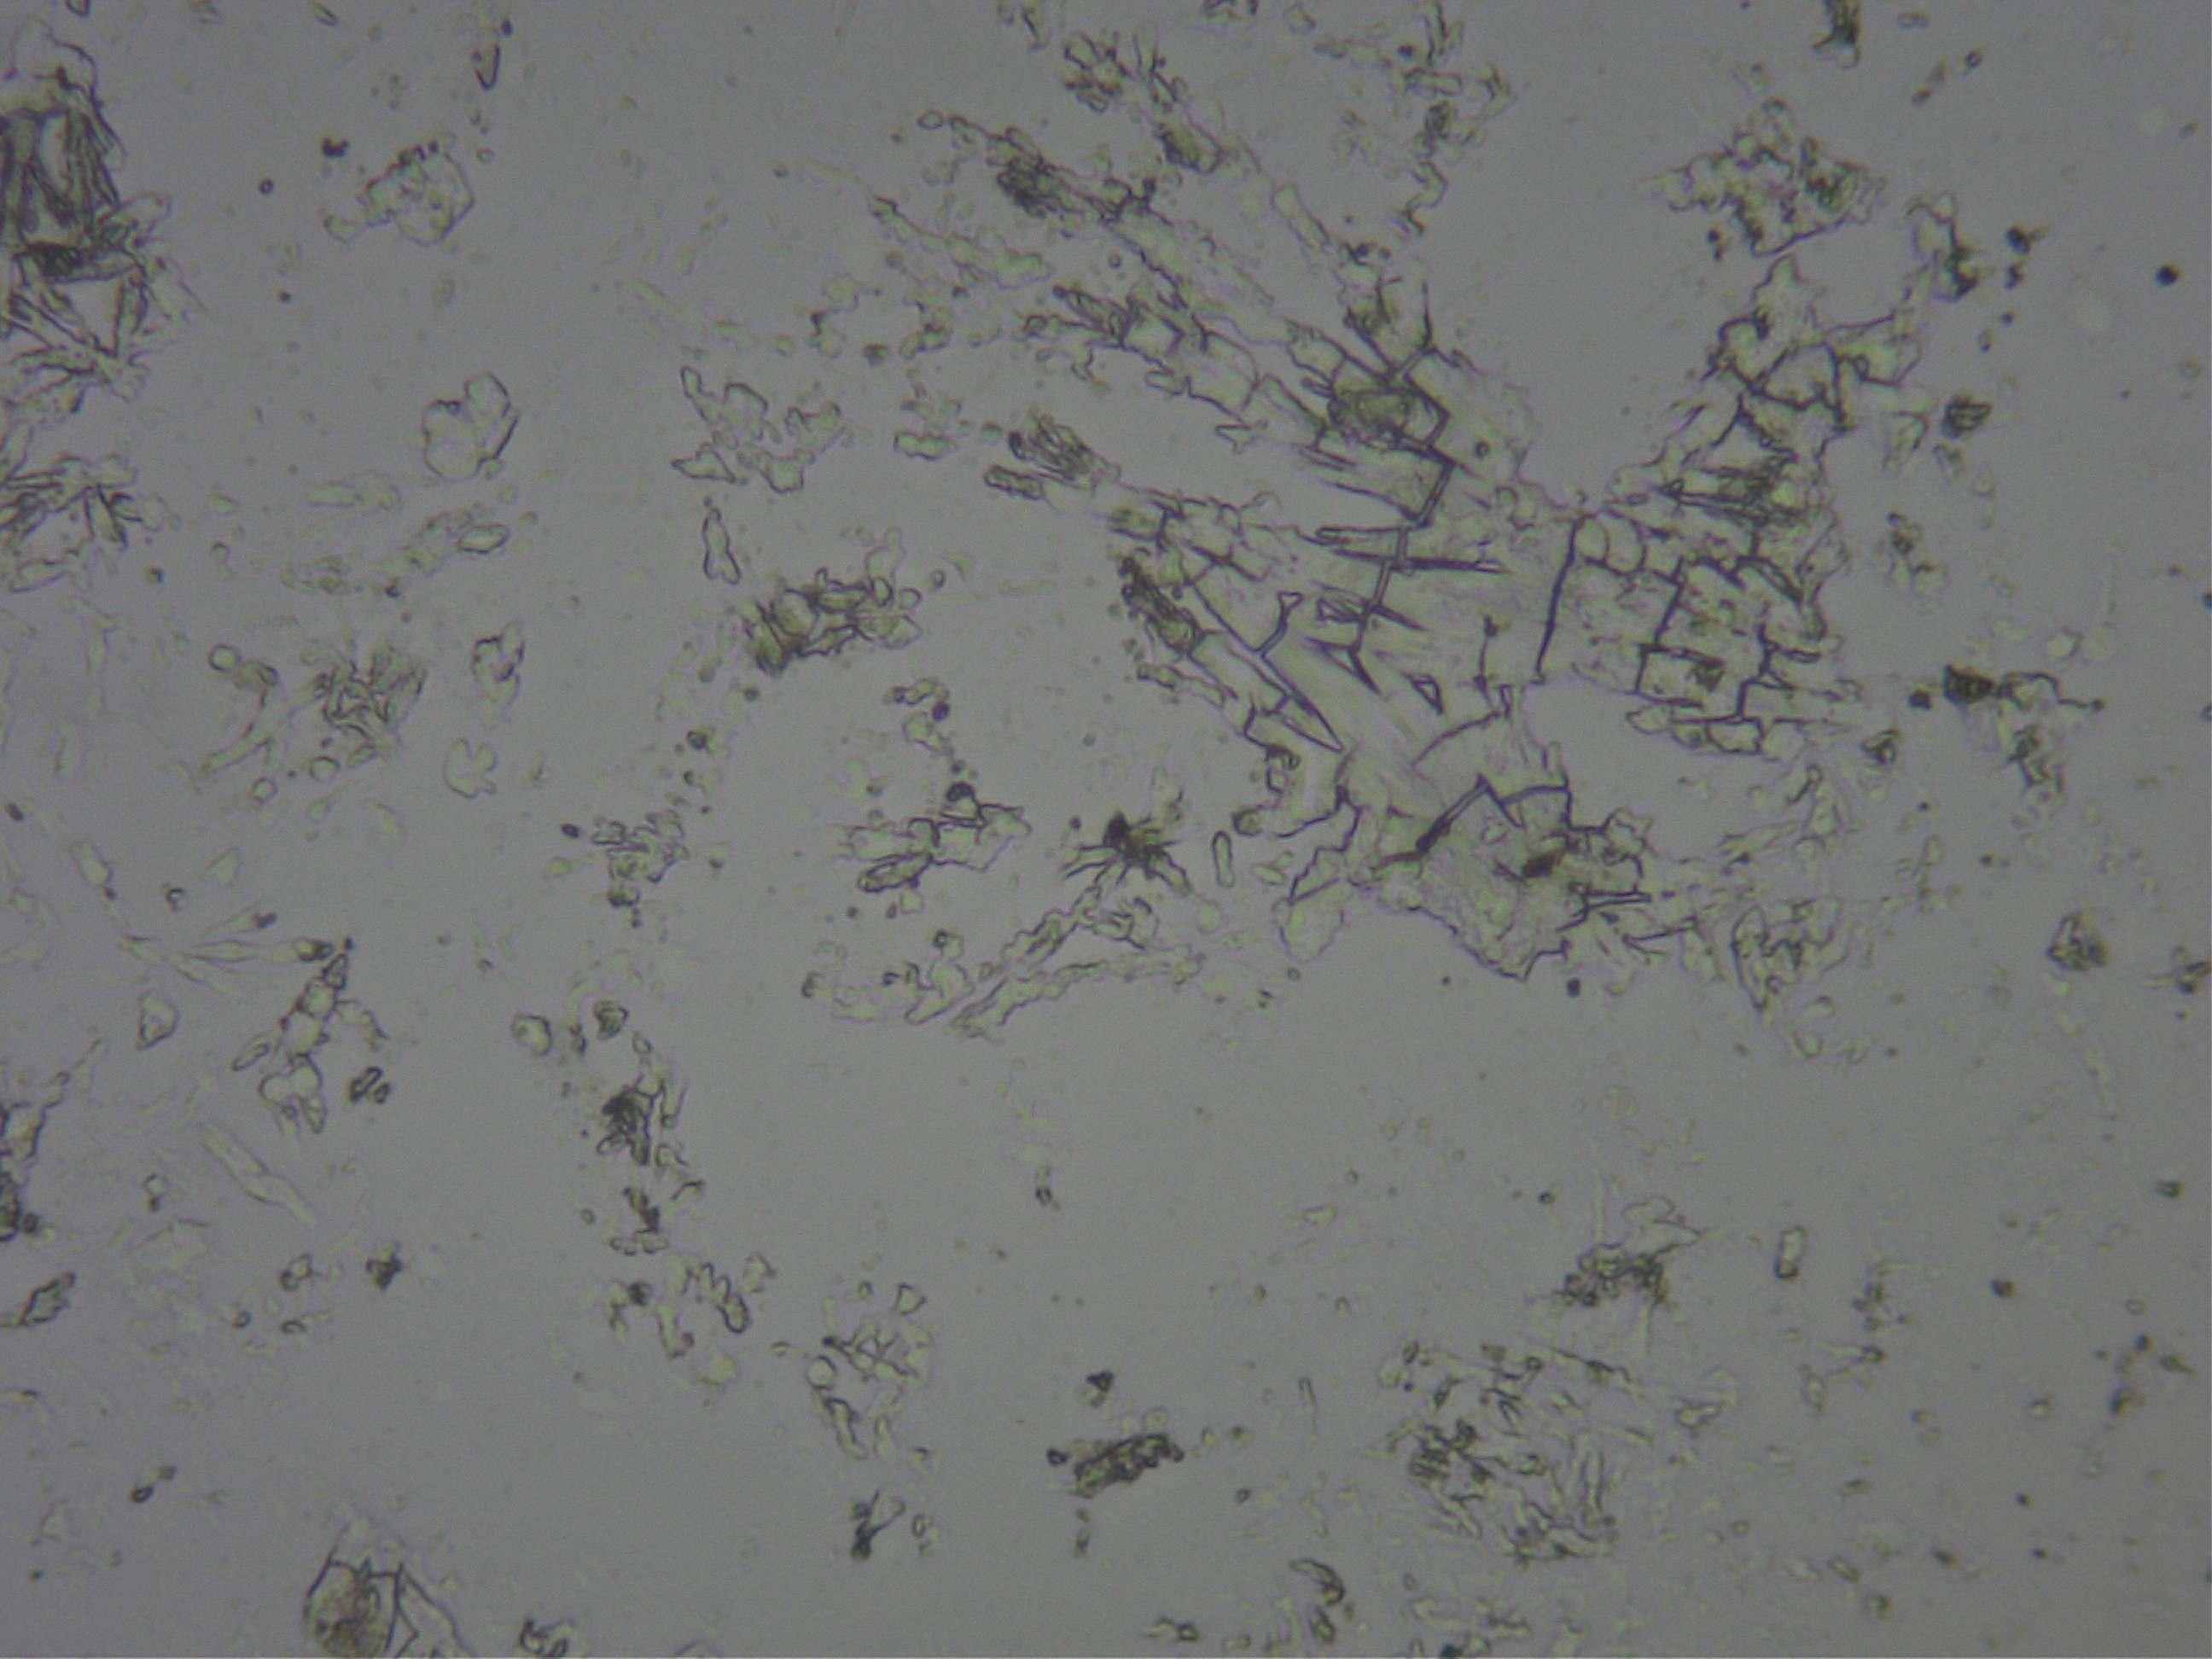
\includegraphics[scale=0.065]{s3.JPG}
    \caption{Light clumps present in thin films}
    \label{fig:light}
  \end{subfigure}
  \caption[HPO images of thin films]{Microstructure images of a thin film taken under HPO ($40\times$ magnification)}
  \label{fig:hpo}
\end{figure}

It can be seen from the images that the volume covered by the particles in the figures are not ordered and distributed randomly, though in clumps.
The distribution of the aggregates was analysed with image analysis.

From subfigures \ref{fig:light} and \ref{fig:dark} there are visible light and dark areas relative to the observed gray area of the glass.
This suggests that there are at least three distinct phases that need to be studied.

\section[Comparison of spatial correlations]{Comparison of two point statistics between probe volumes of a thin film}

Discrete microstructure functions relating the presence of particles and their absence, are derived from image data by means of image segmentation through the Yen binary thresholding method.
Upon studying the two point spatial correlations of microstructures in 12 images, 4 for each type of thin film (S1, S2, S3), it is shown that through principal component analysis that there is no significant difference in the distributions of the particles in the films. Separated contour plots of the data are shown in Figure \ref{fig:cont}.
The contour plots show the regions where the joint probability of finding zinc oxide in the film at two different sites is the same.
From the figures, it can be observed that the variances of the films are large due to the spacing between the lines and that the shapes of the contours are different.
This suggests that the particles are randomly distributed in the substrate. 
It can be also observed that the probability distributions fall abruptly from the center of the plots towards the edges.

From Figure \ref{fig:cont}, the abrupt decrease in the probability of the particles away from a location in the film suggests that there is clumping of materials in the films.
This may mean that there is seed crystalization in the homophobic glass surface in order for the aqueous materials to grow.
Despite the large area used ($225\times 225$ pixels) in calculating the two-point statistics, the distributions are centered around a point suggesting that the distributions of the clumps are sparse. 
This suggests that untreated glass surface is not conducive for crystal adhesion and growth.

\begin{figure}
  \centering
  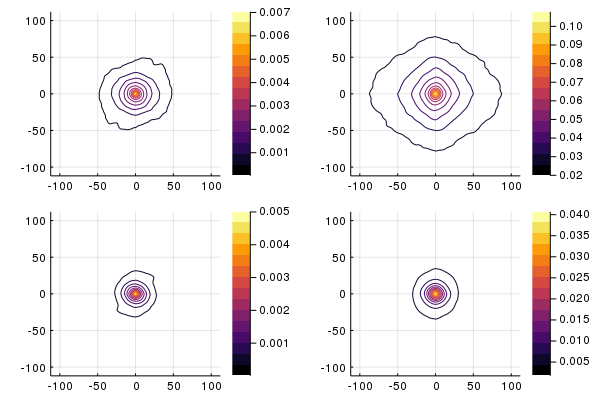
\includegraphics[scale=0.5]{contour.png}
  \caption[Contour plots of spatial correlations]{Contour plots of two point spatial correlations within sections of the same thin film}
  \label{fig:cont}
\end{figure}

\section[Comparison of spatial correlations 2]{Comparison of two point statistics in similar probe volumes of different thin films}

Shown in Figure \ref{fig:pca} are the plots of transformed microstructure function compositions of the particles in the different thin films.
It can be noticed that the plots show that the distributions are random with increasing variance from S1, S2, and S3.
Comparing the particle distributions of films using principal component analysis (Figure \ref{fig:pca}), it can be said that there is no significant difference in the particle distributions relating the presence or absence of material in the films between the three processes; hence, no process-structure properties can be drawn from the results.

\begin{figure}
  \centering
  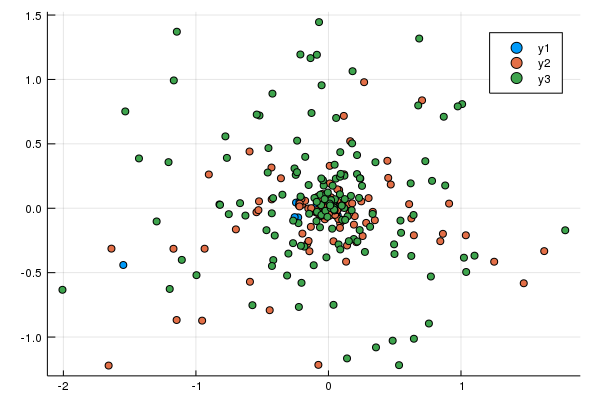
\includegraphics[scale=0.5]{pca.png}
  \caption[Transformed spatial correlations]{Corrected transforms for two-point spatial correlations.}
  \label{fig:pca}
\end{figure}

\section{Results from four-point probe sensing}
The data from four point probe sensing can be summarized by Table \ref{tab:fpsr}.
It can be said that the values follow no rule.
It can also be observed that the half-range values (half of statistical range) follow no pattern.

\begin{table}
  \centering
  \begin{tabular}{c c}
    \toprule
    \multicolumn{2}{c}{S1} \\
    $107.35\pm 24.4$ & $78.5\pm 6.5$ \\
    $243.75\pm 109.4$ & $103.5\pm 0.7$ \\
    \multicolumn{2}{c}{S2} \\
    \midrule
    $146.45 \pm 24.7$ & $181.5\pm 65.2$ \\
    $145.35\pm$ & $254.55\pm 129.6$ \\
    \multicolumn{2}{c}{S3} \\
    \midrule
    $89.8\pm 13.6$ & $159.25\pm 55.6$ \\
    $192.9\pm 32.2$ & $281.2\pm 80.9$ \\
    \bottomrule
  \end{tabular}
  \caption[Four point probe sensing results]{Four point probe sensing voltage drops per thin film section (in mV)}
  \label{tab:fpsr}
\end{table}

Since Table \ref{tab:fpsr} suggests that the four- point probe sensing data are also randomly distributed with large deviations, partial least squares analysis cannot be performed; hence, no strong structure-property relationships can be drawn from the data.
While, a correlation exists ($R^2 = 0.987$) from partial least squares analysis, this may be an overfit left unproven due to the randomness and sparseness of particle distribution.
It is then recommended to use treated glass in boiling diluted sulfuric acid to decrease the randomness and sparseness of film distribution \cite{gao08} to draw stronger correlations \cite{delin} and to further study the crystallinity of the material.
